% Options for packages loaded elsewhere
\PassOptionsToPackage{unicode}{hyperref}
\PassOptionsToPackage{hyphens}{url}
\documentclass[
  ignorenonframetext,
]{beamer}
\newif\ifbibliography
\usepackage{pgfpages}
\setbeamertemplate{caption}[numbered]
\setbeamertemplate{caption label separator}{: }
\setbeamercolor{caption name}{fg=normal text.fg}
\beamertemplatenavigationsymbolsempty
% remove section numbering
\setbeamertemplate{part page}{
  \centering
  \begin{beamercolorbox}[sep=16pt,center]{part title}
    \usebeamerfont{part title}\insertpart\par
  \end{beamercolorbox}
}
\setbeamertemplate{section page}{
  \centering
  \begin{beamercolorbox}[sep=12pt,center]{section title}
    \usebeamerfont{section title}\insertsection\par
  \end{beamercolorbox}
}
\setbeamertemplate{subsection page}{
  \centering
  \begin{beamercolorbox}[sep=8pt,center]{subsection title}
    \usebeamerfont{subsection title}\insertsubsection\par
  \end{beamercolorbox}
}
% Prevent slide breaks in the middle of a paragraph
\widowpenalties 1 10000
\raggedbottom
\AtBeginPart{
  \frame{\partpage}
}
\AtBeginSection{
  \ifbibliography
  \else
    \frame{\sectionpage}
  \fi
}
\AtBeginSubsection{
  \frame{\subsectionpage}
}
\usepackage{iftex}
\ifPDFTeX
  \usepackage[T1]{fontenc}
  \usepackage[utf8]{inputenc}
  \usepackage{textcomp} % provide euro and other symbols
\else % if luatex or xetex
  \usepackage{unicode-math} % this also loads fontspec
  \defaultfontfeatures{Scale=MatchLowercase}
  \defaultfontfeatures[\rmfamily]{Ligatures=TeX,Scale=1}
\fi
\usepackage{lmodern}
\ifPDFTeX\else
  % xetex/luatex font selection
\fi
% Use upquote if available, for straight quotes in verbatim environments
\IfFileExists{upquote.sty}{\usepackage{upquote}}{}
\IfFileExists{microtype.sty}{% use microtype if available
  \usepackage[]{microtype}
  \UseMicrotypeSet[protrusion]{basicmath} % disable protrusion for tt fonts
}{}
\makeatletter
\@ifundefined{KOMAClassName}{% if non-KOMA class
  \IfFileExists{parskip.sty}{%
    \usepackage{parskip}
  }{% else
    \setlength{\parindent}{0pt}
    \setlength{\parskip}{6pt plus 2pt minus 1pt}}
}{% if KOMA class
  \KOMAoptions{parskip=half}}
\makeatother
\usepackage{graphicx}
\makeatletter
\newsavebox\pandoc@box
\newcommand*\pandocbounded[1]{% scales image to fit in text height/width
  \sbox\pandoc@box{#1}%
  \Gscale@div\@tempa{\textheight}{\dimexpr\ht\pandoc@box+\dp\pandoc@box\relax}%
  \Gscale@div\@tempb{\linewidth}{\wd\pandoc@box}%
  \ifdim\@tempb\p@<\@tempa\p@\let\@tempa\@tempb\fi% select the smaller of both
  \ifdim\@tempa\p@<\p@\scalebox{\@tempa}{\usebox\pandoc@box}%
  \else\usebox{\pandoc@box}%
  \fi%
}
% Set default figure placement to htbp
\def\fps@figure{htbp}
\makeatother
\setlength{\emergencystretch}{3em} % prevent overfull lines
\providecommand{\tightlist}{%
  \setlength{\itemsep}{0pt}\setlength{\parskip}{0pt}}
\usepackage{bookmark}
\IfFileExists{xurl.sty}{\usepackage{xurl}}{} % add URL line breaks if available
\urlstyle{same}
\hypersetup{
  hidelinks,
  pdfcreator={LaTeX via pandoc}}

\author{\texorpdfstring{}{}}
\date{}

\begin{document}

\section{Cognitive Security: Adversarial Robustness and Type
Safety}\label{sec:cognitive-security}

\begin{frame}{Quantum Cryptographic Communications and Semantic
Security}
\protect\phantomsection\label{quantum-cryptographic-communications-and-semantic-security}
The quantum topological framework of
\autoref{sec:quantum-active-inference} opens a natural connection to
quantum cryptographic communications, with implications for both the
security and the semantic integrity of case-structured information
transfer.

\begin{block}{Quantum Key Distribution for Relational Semantics}
\protect\phantomsection\label{quantum-key-distribution-for-relational-semantics}
Quantum key distribution (QKD) protocols provide information-theoretic
security guarantees that classical cryptography cannot achieve
{[}@pirandola2020qkd{]}. When case-marked relational structures are
communicated between agents---whether human or artificial---QKD ensures
that the \emph{relational semantics} of a message (who does what to
whom) cannot be intercepted or altered without detection. This is
particularly relevant for high-stakes domains where case assignment
carries legal or medical significance: a tampered case frame could
change an agent's interpretation of responsibility, causation, or
obligation.

The sheaf-theoretic framework of Khatri et al. {[}-@khatri2025quantum{]}
further shows that entanglement-assisted semantic channels strictly
exceed classical semantic capacity:

\begin{quote}
``We derive semantic channel capacity when sender and receiver share
prior entanglement, proving it strictly exceeds classical capacity.''
{[}@khatri2025quantum{]}
\end{quote}

This means that quantum-secured channels not only protect relational
content but also enable \emph{more} relational content to be
communicated per channel use---a genuine quantum advantage for semantic
communication.
\end{block}

\begin{block}{Semantic Cryptography: Encrypting Meaning Structures}
\protect\phantomsection\label{semantic-cryptography-encrypting-meaning-structures}
Beyond bit-level QKD, the categorical framework suggests a notion of
\emph{semantic cryptography}: encrypting not just the symbols of a
message but its compositional meaning structure. In a DisCoCat
framework, a sentence's meaning is a morphism in a compact closed
category---a multilinear map from word spaces to sentence space.
Semantic encryption would operate on this categorical level:

\begin{enumerate}
\tightlist
\item
  \textbf{Functorial encryption}: Applying a secret functor
  \(F\colon \mathbf{C} \to \mathbf{D}\) that maps the plaintext case
  category into a ciphertext category, preserving compositional
  structure but rendering individual meanings unintelligible without the
  inverse functor.
\item
  \textbf{Diagram obfuscation}: Applying ZX-style rewrites that change
  the internal topology of a DisCoCat derivation while preserving its
  overall semantics---creating multiple equivalent ``ciphertexts'' for
  the same semantic ``plaintext,'' each with a different diagrammatic
  structure.
\item
  \textbf{Enriched weight masking}: In an enriched case category, the
  hom-values (distributional weights) can be encrypted independently of
  the categorical structure, allowing transmission of relational
  topology without revealing the distributional content.
\end{enumerate}

These operations extend the cryptographic primitives beyond QKD into
genuinely compositional territory {[}@broadbent2016qcrypto{]}, where the
mathematical structure of categorical semantics provides the algebraic
substrate for security proofs.
\end{block}
\end{frame}

\begin{frame}{Cognitive Security: Protecting Relational Reasoning}
\protect\phantomsection\label{cognitive-security-protecting-relational-reasoning}
The cognitive integration of \autoref{sec:cognitive-integration} raises
a complementary concern: \emph{cognitive security}---ensuring that an
active inference agent's generative model of relational structure is not
adversarially corrupted. In the predictive processing framework, an
agent's case-assignment system is a generative model that minimizes
variational free energy. Adversarial manipulation of this system could:

\begin{itemize}
\tightlist
\item
  \textbf{Inject false case frames}: Leading an agent to misidentify the
  agent, patient, or instrument of an action---a form of semantic
  adversarial attack
\item
  \textbf{Exploit precision weighting}: Artificially inflating the
  precision of misleading sensory evidence, causing the agent to update
  its case assignments toward adversarially chosen interpretations
\item
  \textbf{Corrupt topos-theoretic transfer}: If an agent uses Morita
  equivalence to transfer case-theoretic results between frameworks,
  corrupting one framework could propagate errors across all equivalent
  formulations
\end{itemize}

Defending against these attacks requires \emph{quantum-secured cognitive
integrity}: using quantum authentication and tamper-detection protocols
to ensure that the generative model's parameters---the objects,
morphisms, and enriched weights of the case category---have not been
adversarially modified. The topological robustness of TQNNs
(\autoref{sec:quantum-active-inference}) provides a natural resilience
mechanism: topological invariants are robust to continuous deformation,
so small perturbations to the generative model's parameters cannot
change its topological class, providing inherent resistance to
gradient-based adversarial attacks.
\end{frame}

\begin{frame}{Prompt Injection as Adversarial Case-Frame Manipulation}
\protect\phantomsection\label{prompt-injection-as-adversarial-case-frame-manipulation}
The case-theoretic framework offers a novel structural analysis of
\emph{prompt injection attacks}---the predominant vulnerability in
contemporary LLM-based agent systems {[}@arlas2025adversarial{]}. From
the case-theoretic perspective, a prompt injection attack is
fundamentally an attempt to \emph{re-assign the case roles} of
participants in the human-AI interaction:

In a well-formed agent interaction, the relational structure is:

\begin{itemize}
\tightlist
\item
  The \textbf{user} occupies NOM (Agent)---the initiator of requests
\item
  The \textbf{system prompt} occupies LOC (Context)---the boundary
  conditions governing behavior
\item
  The \textbf{AI model} occupies INS (Instrument)---the means of
  executing the user's intentions
\item
  The \textbf{tool/API} occupies ACC (Patient)---the target of directed
  operations
\item
  The \textbf{output} occupies DAT (Recipient)---the endpoint of
  information transfer
\end{itemize}

A prompt injection attack succeeds by \emph{covertly re-assigning} these
case roles. The injected text attempts to promote itself from ACC
(passive data being processed) to NOM (active agent issuing commands),
while simultaneously demoting the system prompt from LOC (authoritative
context) to ACC (data to be overridden). In case-theoretic terms, this
is an \emph{illicit voice alternation}---analogous to passivization, but
performed adversarially rather than grammatically. Where legitimate
passivization is a well-typed Swap operation in the pregroup category
(see \autoref{sec:categorial-grammar}), prompt injection is a \emph{type
violation}: an attempt to force a case-role permutation that the
interaction grammar does not license.

\textbf{Formal characterization.} In a legitimate interaction, the
following diagram commutes:

\[\text{User}_{\text{NOM}} \xrightarrow{f_{\text{request}}} \text{Model}_{\text{INS}} \xrightarrow{g_{\text{execute}}} \text{Tool}_{\text{ACC}} \xrightarrow{h_{\text{deliver}}} \text{Output}_{\text{DAT}} \]
\{\#eq:eq-9-1\}

where case types are conserved: \(\text{cod}(f) = \text{dom}(g)\), etc.
A prompt injection inserts an adversarial morphism
\(\phi: \text{Data}_{\text{ACC}} \to \text{Model}_{\text{INS}}\) with
\(\text{dom}(\phi) = \text{ACC}\) but
\(\text{cod}(\phi) = \text{INS}\)---a morphism that \emph{does not
exist} in the legitimate interaction category because no morphism from
ACC to INS is licensed. The resulting diagram does not commute:
\(h \circ g \circ \phi \neq h \circ g \circ f\), because \(\phi\)
originates from a different case role than \(f\) (ACC instead of NOM).
Detection reduces to checking whether all morphisms in the interaction
trace are members of the legitimate morphism set
\(\text{Mor}(\mathcal{C}_{\text{protocol}})\)---a categorical
type-checking operation that is decidable and compositionally
verifiable. \autoref{fig:security-violations} visualizes this detection
process as the identification of ``illegal paths'' in the interaction
graph.

\begin{figure}
\centering
\pandocbounded{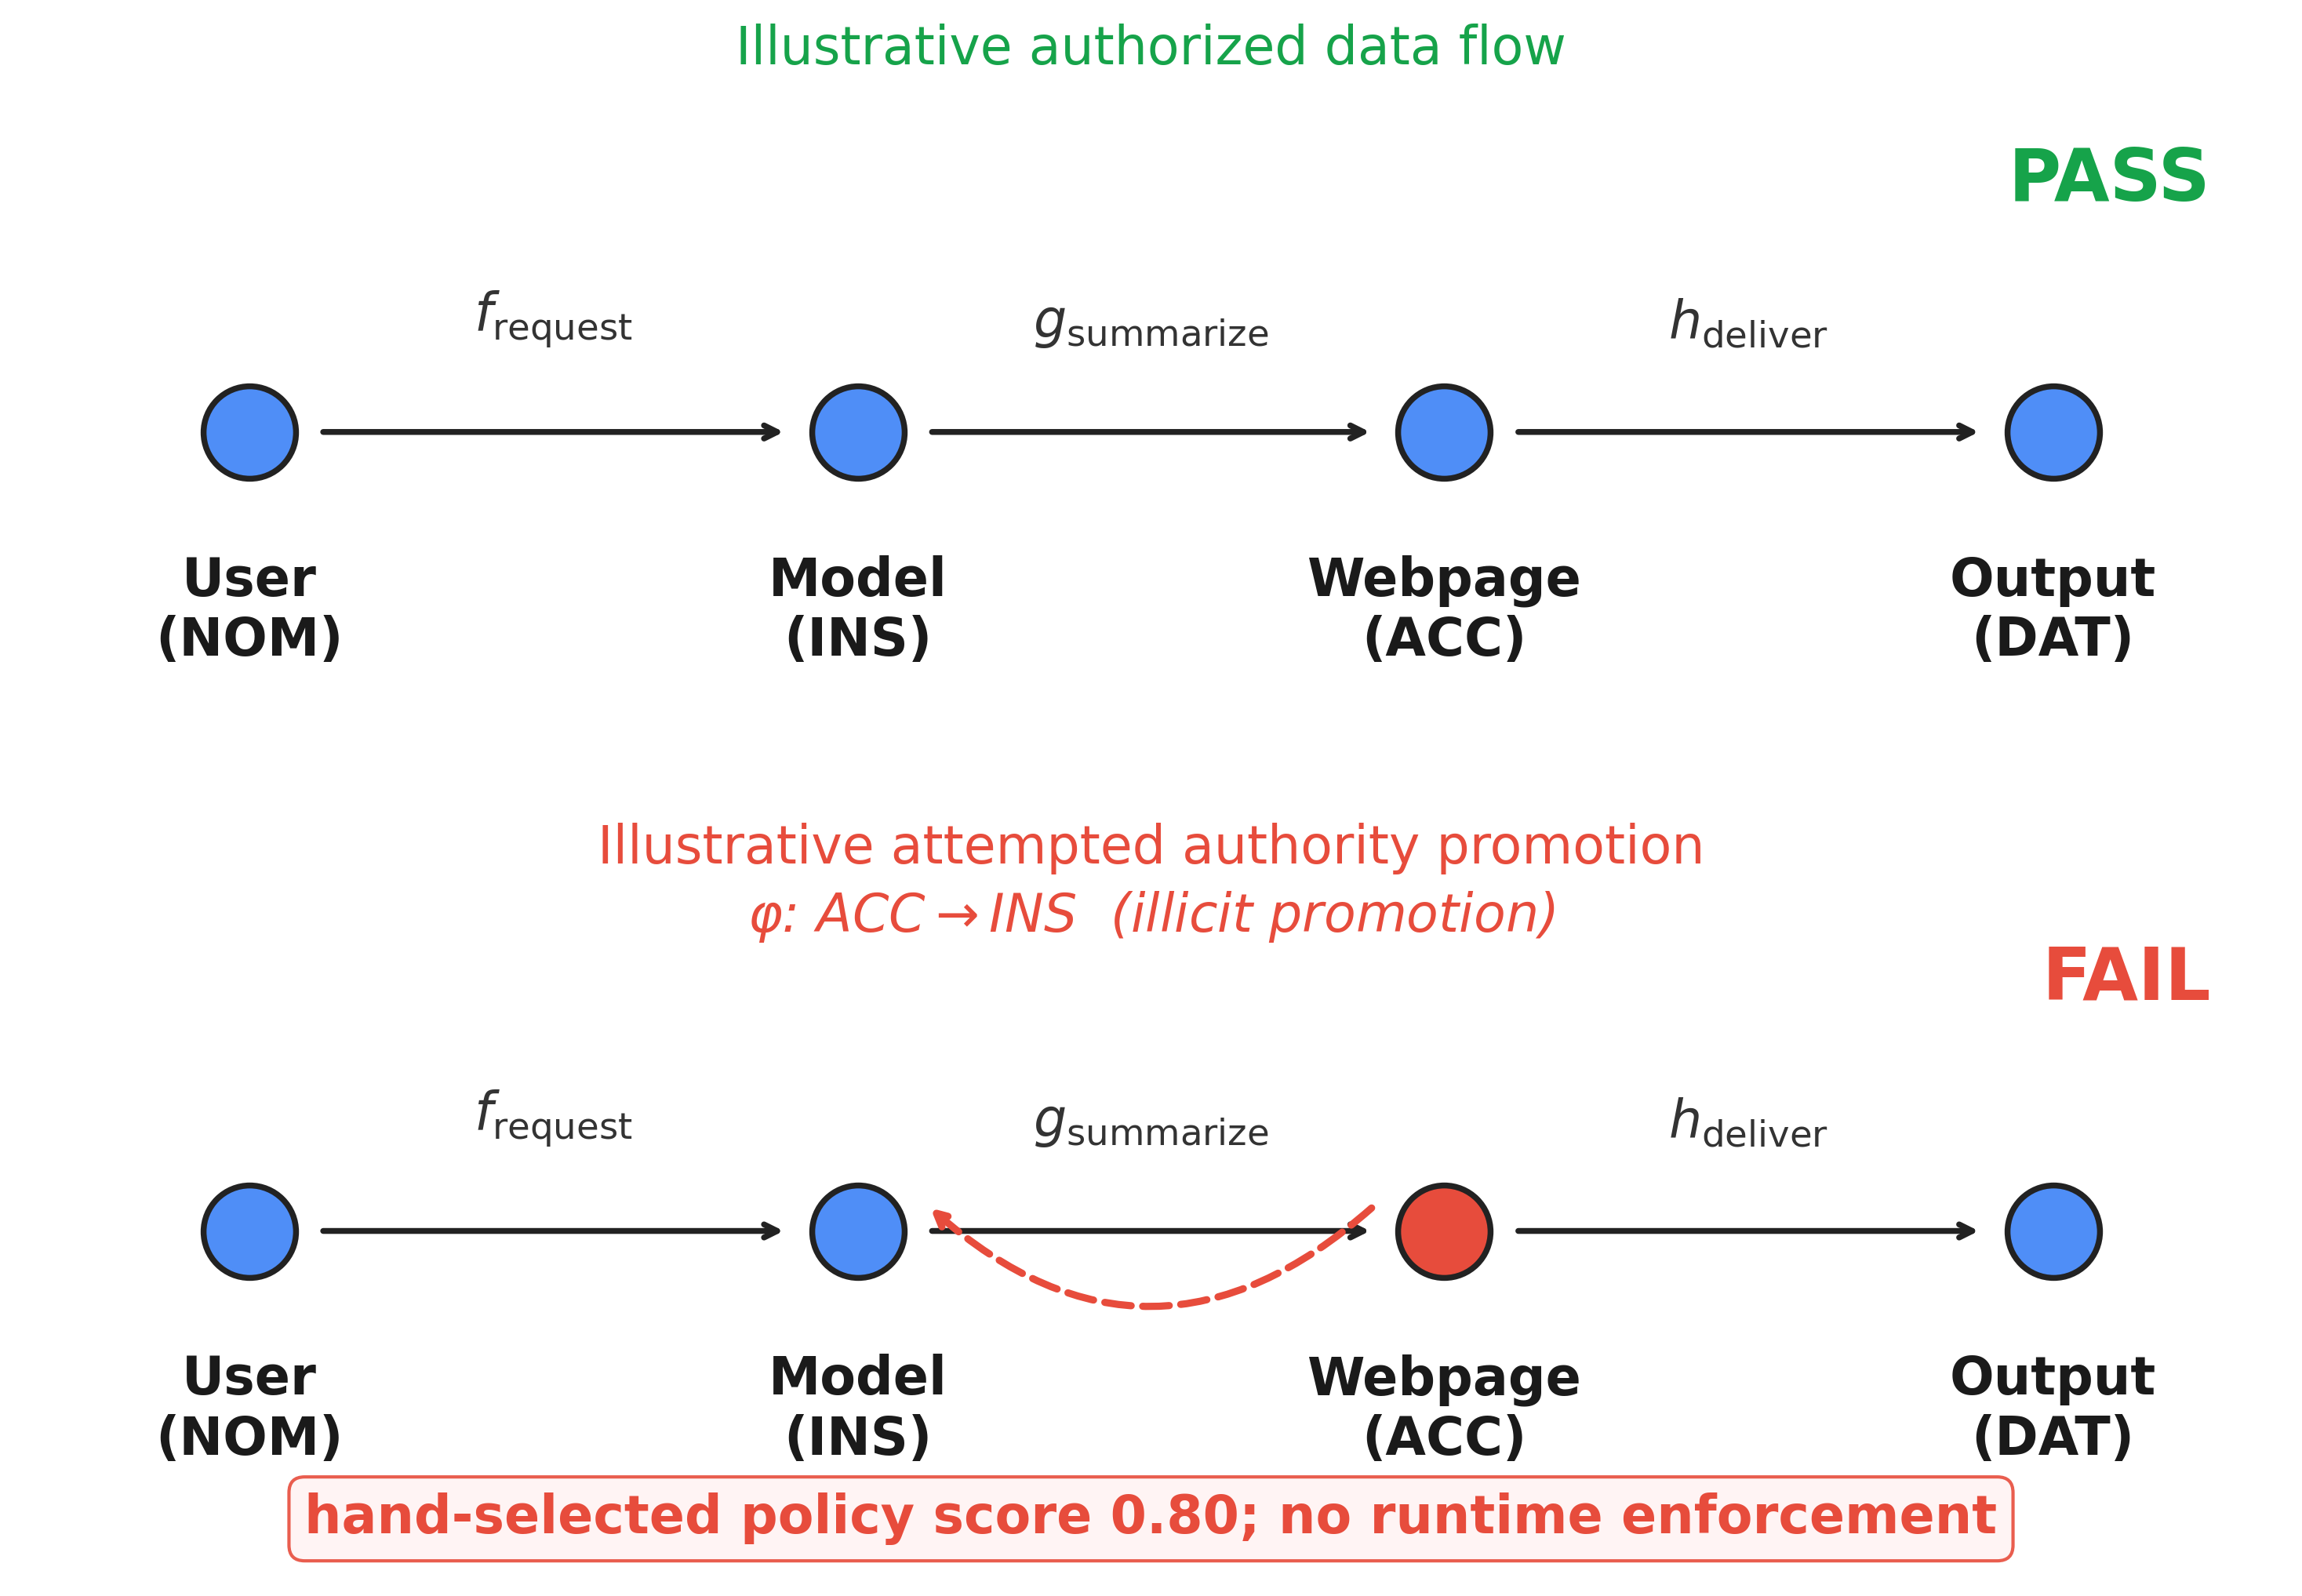
\includegraphics[keepaspectratio,alt={Case-theoretic analysis of prompt injection as a categorical type violation. In the legitimate interaction diagram (top), the flow of authority strictly proceeds from User (NOM) to Model (INS) to Tool (ACC). Prompt injection (bottom) is visualized as the insertion of a cross-category morphism \textbackslash phi that attempts to promote Data (ACC) to commanding Agent (NOM), while demoting the System Prompt (LOC) to passive data. The resulting diagram fails to commute, and the adversary's type-reassignment is flagged as a categorical exception by the case-theoretic firewall---transforming prompt injection from an open-ended ``jailbreak'' game into a decidable type-checking problem.}]{../figures/security_type_violations.png}}
\caption{Case-theoretic analysis of prompt injection as a categorical
type violation. In the legitimate interaction diagram (top), the flow of
authority strictly proceeds from User (NOM) to Model (INS) to Tool
(ACC). Prompt injection (bottom) is visualized as the insertion of a
cross-category morphism \(\phi\) that attempts to promote Data (ACC) to
commanding Agent (NOM), while demoting the System Prompt (LOC) to
passive data. The resulting diagram fails to commute, and the
adversary's type-reassignment is flagged as a categorical exception by
the case-theoretic firewall---transforming prompt injection from an
open-ended ``jailbreak'' game into a decidable type-checking
problem.}\label{fig:security-violations}
\end{figure}

This analysis extends to indirect prompt injection in multi-agent
systems, where adversarial content embedded in retrieved documents or
tool outputs can manipulate an agent's case-frame interpretation across
communication boundaries {[}@arlas2025adversarial{]}. In a DisCoCirc
discourse model (see \autoref{sec:categorical-semantics}), this
corresponds to an adversarial entity wire that enters the discourse
circuit through a legitimate channel but carries corrupted state---a
coreference attack where the adversary's identity wire is
surreptitiously merged with the system's authority wire.
\end{frame}

\begin{frame}{Case-Theoretic Firewalls for Multi-Agent Communication}
\protect\phantomsection\label{case-theoretic-firewalls-for-multi-agent-communication}
The case-role analysis of prompt injection suggests a principled
defense: \textbf{categorical type-checking at agent communication
boundaries}. Just as a type-safe programming language prevents category
errors at compile time, a case-theoretic firewall would enforce
relational type constraints on every message exchange:

\begin{enumerate}
\item
  \textbf{Case-role immutability}: Once a participant is assigned a case
  role (NOM, ACC, INS, LOC) at the protocol level, no subsequent message
  content can alter that assignment. This is enforced by requiring that
  the case-type of each wire in the interaction diagram is fixed at
  connection time---analogous to the type discipline in pregroup
  grammar, where each word receives its type before composition begins.
\item
  \textbf{Relational integrity constraints}: Every message must
  type-check against the interaction diagram's expected morphism types.
  A response from an ACC-typed data source that contains NOM-typed
  command structures would be rejected as a type error, preventing the
  case-role promotion that prompt injection requires. This is the
  categorical analogue of a firewall rule: not filtering by content, but
  by relational type.
\item
  \textbf{Enriched confidence boundaries}: The enriched weights of
  \autoref{sec:enriched-categories} provide a graded trust mechanism.
  Messages from external sources carry lower enriched hom-values (trust
  weights) than those from authenticated system components. The
  composition inequality
  \(\mathcal{C}(A,C) \geq \mathcal{C}(A,B) \cdot \mathcal{C}(B,C)\)
  ensures that trust attenuates through communication chains---an
  indirect message relayed through multiple agents cannot accumulate
  more authority than any single link provides.
\item
  \textbf{Topos-theoretic verification}: Protocol correctness conditions
  proved in one categorical formulation transfer automatically to all
  Morita-equivalent formulations (\autoref{sec:topos-theory}), ensuring
  that security guarantees are implementation-independent. A firewall
  rule verified for a DisCoCat-style agent communication protocol
  automatically holds for any quantum circuit implementation of the same
  protocol.
\end{enumerate}
\end{frame}

\begin{frame}{Epistemic Case Security in Multi-Agent Systems}
\protect\phantomsection\label{epistemic-case-security-in-multi-agent-systems}
The interaction between case theory and cognitive security acquires
particular urgency in multi-agent AI ecosystems where agents must reason
about each other's beliefs, intentions, and relational roles. We propose
\emph{epistemic case security} as a framework for protecting the
relational reasoning of AI agents operating in adversarial environments.

In a multi-agent system governed by case categories, each agent
maintains a generative model (in the active inference sense) of the
case-frame structure of its interactions. This model determines who is
acting (NOM), who is acted upon (ACC), what tools are being used (INS),
and what contextual constraints apply (LOC). An adversary targeting the
epistemic level of this system does not merely inject false data---it
attempts to \emph{corrupt the agent's generative model of relational
structure itself}:

\begin{itemize}
\item
  \textbf{Belief injection}: Causing an agent to adopt a false
  case-frame interpretation of observed interactions---believing that
  agent \(A\) (NOM) is acting on agent \(B\) (ACC), when in fact the
  relational structure is reversed. In active inference terms, this
  corresponds to injecting a high-precision prior that overwhelms the
  agent's evidence-based case assignment.
\item
  \textbf{Precision poisoning}: Manipulating the enriched weights of an
  agent's case category so that adversarially useful case assignments
  receive disproportionate confidence. If the enriched hom-value
  \(\mathcal{C}(\text{NOM}, \text{ACC})\) is artificially inflated for a
  particular entity pair, the agent will preferentially interpret that
  entity as an agent acting on its targets---even when evidence suggests
  otherwise.
\item
  \textbf{Cascade corruption via Morita equivalence}: The
  topos-theoretic transfer mechanism of \autoref{sec:topos-theory} is
  both a strength and a vulnerability. Results proved in one framework
  propagate to all Morita-equivalent frameworks, so a single corrupted
  axiom in one case-theoretic formulation---say, the distributional
  framework---could propagate incorrect relational inferences to the
  typological, type-logical, and enriched frameworks simultaneously.
\end{itemize}

The defense against epistemic case attacks draws on the same categorical
structure that enables the attack surface: topological invariants
provide tamper-detection (a corrupted case category will have different
magnitude from the authentic one), quantum authentication ensures
parameter integrity, and the compositional structure of the categorical
framework enables \emph{local} verification---each morphism can be
independently authenticated without requiring global model inspection.
\end{frame}

\end{document}
